%\documentclass{beamer}
%\documentclass[slidestop,usepdftitle=false]{beamer}
\documentclass[english,10pt,table]{beamer}
%\documentclass[english,10pt,table,handout]{beamer}
% Copyright 2007 by Till Tantau
%
% This file may be distributed and/or modified
%
% 1. under the LaTeX Project Public License and/or
% 2. under the GNU Public License.
%
% See the file doc/licenses/LICENSE for more details.


% Common packages

\usepackage[english]{babel}
\usepackage[utf8]{vietnam}
%\usepackage{times}
\usefonttheme[onlymath]{serif}
\usecolortheme{default}
\usepackage{booktabs}
\usepackage{mathpartir}
\usepackage{listings}
\usepackage{pbox}
\mprset{flushleft}
\mode<article>
{
  \usepackage{times}
  \usepackage{mathptmx}
  \usepackage[left=1.5cm,right=6cm,top=1.5cm,bottom=3cm]{geometry}
}

\usepackage{hyperref}
\usepackage{tikz}
\usetikzlibrary{arrows,backgrounds}
%\tikzstyle{mnode}=[circle, draw, fill=black, inner sep=0pt, minimum width=4pt]
\usepackage{colortbl}
%\usepackage{yfonts}
\usepackage{translator} % comment this, if not available


% Common settings for all lectures in this course

\def\lecturename{HCMUT H6 - Building}
\def\insertdate{20/06/2021}

\title{\insertlecture}

\author{H.Đ.Hưng,L.T.Nguyên, H.V.Đức,N.T.Trọng, N.T.Nam}

\institute
{
    %\textbf{Trường Đại Học Bách Khoa - ĐHQG TP.HCM}
  \textbf{Trường đại học Bách khoa - ĐHQG HCM} \\
  Khoa khoa học và kỹ thuật máy tính\\
	\textcolor{blue}{\{hung.hoduccse,trong.ngo08082002,trong.ngo08082002,\\
	trong.ngo08082002,trong.ngo08082002\}@hcmut.edu.vn}
}

\subject{Lecturer \lecturename}




% Beamer version theme settings

\useoutertheme[height=0pt,width=2cm,right]{sidebar}
\usecolortheme{rose,sidebartab}
\useinnertheme{circles}
\usefonttheme[only large]{structurebold}

\setbeamercolor{sidebar right}{bg=black!15}
\setbeamercolor{structure}{fg=blue}
\setbeamercolor{author}{parent=structure}

\setbeamerfont{title}{series=\normalfont,size=\LARGE}
\setbeamerfont{title in sidebar}{series=\bfseries}
\setbeamerfont{author in sidebar}{series=\bfseries}
\setbeamerfont*{item}{series=}
\setbeamerfont{frametitle}{size=}
\setbeamerfont{block title}{size=\small}
\setbeamerfont{subtitle}{size=\normalsize,series=\normalfont}

\setbeamertemplate{navigation symbols}{}
\setbeamertemplate{bibliography item}[book]
\setbeamertemplate{sidebar right}
{
  {\usebeamerfont{title in sidebar}%
    \vskip1.5em%
    \hskip3pt%
    \usebeamercolor[fg]{title in sidebar}%
    \insertshorttitle[width=2cm,center,respectlinebreaks]\par%
    \vskip1.25em%
  }%
  {%
    \hskip3pt%
    \usebeamercolor[fg]{author in sidebar}%
    \usebeamerfont{author in sidebar}%
    \insertshortauthor[width=2cm,center,respectlinebreaks]\par%
    \vskip1.25em%
  }%
  \hbox to2cm{\hss\insertlogo\hss}
  \vskip1.25em%
  \insertverticalnavigation{2cm}%
  \vfill
  \hbox to 2cm{\hfill\usebeamerfont{subsection in
      sidebar}\strut\usebeamercolor[fg]{subsection in
      sidebar}\insertshortlecture.\insertframenumber\hskip5pt}%
  \vskip3pt%
}%

\setbeamertemplate{title page}
{
  \vbox{}
  \vskip1em
  {\huge \textbf{Lập trình nâng cao}\\}
  {\usebeamercolor[fg]{title}\usebeamerfont{title}\inserttitle\par}%
  \ifx\insertsubtitle\@empty%
  \else%
    \vskip0.25em%
    {\usebeamerfont{subtitle}\usebeamercolor[fg]{subtitle}\insertsubtitle\par}%
  \fi%     
  \vskip1em\par
  {\Large\color{blue}\textbf{Design Pattern: Strategy}\\}
  \vskip1em\par
  \emph{\lecturename}\ on \insertdate\par
  \vskip0pt plus1filll
  \leftskip=0pt plus1fill\insertauthor\par
  \insertinstitute\vskip1em
}

\logo{
\includegraphics[width=1.5cm]{hcmut.png}}



% Article version layout settings

\mode<article>

\makeatletter
\def\@listI{\leftmargin\leftmargini
  \parsep 0pt
  \topsep 5\p@   \@plus3\p@ \@minus5\p@
  \itemsep0pt}
\let\@listi=\@listI


\setbeamertemplate{frametitle}{\paragraph*{\insertframetitle\
    \ \small\insertframesubtitle}\ \par
}
\setbeamertemplate{frame end}{%
  \marginpar{\scriptsize\hbox to 1cm{\sffamily%
      \hfill\strut\insertshortlecture.\insertframenumber}\hrule height .2pt}}
\setlength{\marginparwidth}{1cm}
\setlength{\marginparsep}{4.5cm}

\def\@maketitle{\makechapter}

\def\makechapter{
  \newpage
  \null
  \vskip 2em%
  {%
    \parindent=0pt
    \raggedright
    \sffamily
    \vskip8pt
    {\fontsize{36pt}{36pt}\selectfont Chapter \insertshortlecture \par\vskip2pt}
    {\fontsize{24pt}{28pt}\selectfont \color{blue!50!black} \insertlecture\par\vskip4pt}
    {\Large\selectfont \color{blue!50!black} \insertsubtitle\par}
    \vskip10pt

    \normalsize\selectfont Print version of
    Lecturer \emph{\lecturename} of \@date\par\vskip1.5em
    \hfill Hung Duc Ho, Faculty of CSE, University of Technology
  }
  \par
  \vskip 1.5em%
}

\let\origstartsection=\@startsection
\def\@startsection#1#2#3#4#5#6{%
  \origstartsection{#1}{#2}{#3}{#4}{#5}{#6\normalfont\sffamily\color{blue!50!black}\selectfont}}

\makeatother

\mode
<all>




% Typesetting Listings
\usepackage[framemethod=TikZ]{mdframed}
\usepackage{amsthm}
\usepackage[utf8]{vietnam}

\usepackage{xcolor}
\usepackage{listings}

\colorlet{mygray}{black!30}
\colorlet{mygreen}{green!60!blue}
\colorlet{mymauve}{red!60!blue}

\lstset{
  backgroundcolor=\color{gray!10},  
  basicstyle=\ttfamily,
  columns=fullflexible,
  breakatwhitespace=false,      
  breaklines=true,                
  captionpos=b,                    
  commentstyle=\color{mygreen},
  extendedchars=true,              
  frame=single,  
  keepspaces=true,             
  keywordstyle=\color{blue},      
  language=C++,
  numbers=none,                
  numbersep=5pt,                   
  numberstyle=\tiny\color{blue}, 
  rulecolor=\color{mygray},        
  showspaces=false,               
  showtabs=false,                 
  stepnumber=5,                  
  stringstyle=\color{mygreen},    
  tabsize=3,                      
  title=\lstname                
}
%\lstset{language=C++}

%\alt<presentation>
%{\lstset{%
%  basicstyle=\footnotesize\ttfamily,
%  commentstyle=\slshape\color{green!50!black},
%  keywordstyle=\bfseries\color{blue!50!black},
%  identifierstyle=\color{blue},
%  stringstyle=\color{orange},
%  escapechar=\#,
%  emphstyle=\color{red}}
%}
%{
%  \lstset{%
%    basicstyle=\ttfamily,
%    keywordstyle=\bfseries,
%    commentstyle=\itshape,
%   escapechar=\#,
%    emphstyle=\bfseries\color{red}
%  }
%}

% Common theorem-like environments

\theoremstyle{example}
\newtheorem{exercise}[theorem]{\translate{Exercise}}


% New useful definitions:

\newbox\mytempbox
\newdimen\mytempdimen

\newcommand\includegraphicscopyright[3][]{%
  \leavevmode\vbox{\vskip3pt\raggedright\setbox\mytempbox=\hbox{\includegraphics[#1]{#2}}%
    \mytempdimen=\wd\mytempbox\box\mytempbox\par\vskip1pt%
    \fontsize{3}{3.5}\selectfont{\color{black!25}{\vbox{\hsize=\mytempdimen#3}}}\vskip3pt%
}}

\newenvironment{colortabular}[1]{\medskip\rowcolors[]{1}{blue!20}{blue!10}\tabular{#1}\rowcolor{blue!40}}{\endtabular\medskip}

\def\equad{\leavevmode\hbox{}\quad}

\newenvironment{greencolortabular}[1]
{\medskip\rowcolors[]{1}{green!50!black!20}{green!50!black!10}%
  \tabular{#1}\rowcolor{green!50!black!40}}%
{\endtabular\medskip}



\lecture[CO2039]{\textbf{C02039 - HK212 \quad}}{lecture-text}

\usepackage{pifont}
\usepackage{color}
%%%%%%%%%%%%%%%%%%%%%%%%

%%%%%%%%%%%%%%%%%%%%%%%%

% Symbol definitions for these lists
\newcommand{\DingListSymbolA}{43}
\newcommand{\DingListSymbolB}{243}
\newcommand{\DingListSymbolC}{224}
\newcommand{\DingListSymbolD}{219}

% Boxed equation
\definecolor{LightYellow}{rgb}{1.,1.,.9}
\definecolor{LightRed}{rgb}{1.,.6,.6}


%%ensembles de nombres
\def\NP{$\mathcal{NP}$}
\def\N{\mathbb{N}}
\def\Z{\mathbb{Z}}
\def\R{\mathbb{R}}
\def\Q{\mathbb{Q}}

%\date[]{~~}
%%%%%%%%%%%%%%%%%%%%%%%%%%%%%%%%%%%%%%%%%%%%%%%%%%%%%%%%%%%%%%%%%%%%%
%%%%%%%%%%%%%%%%%%%%%%%%%%%%%%%%%%%%%%%%%%%%%%%%%%%%%%%%%%%%%%%%%%%%%
\begin{document}



\frame{
\selectlanguage{english}
  \maketitle
}


%%%%%%%%%%%%%%%%%%%%%%%%%%%%%%%%%%%%%%%%%%%%%%%%%%%%%%%%%%%%%%%%%%%%%
%%%%%%%%%%%%%%%%%%%%%%%%%%%%%%%%%%%%%%%%%%%%%%%%%%%%%%%%%%%%%%%%%%%%%
%\section[Plan]{}
%\setcounter{tocdepth}{1}
\frame{ \tableofcontents}
%\setcounter{tocdepth}{5}
% to display left summary deeper and plan slide juste display section: add command \setcounter{tocdepth}{1} and then \setcounter{tocdepth}{10}  recompile twice or more again 

%%%%%%%%%%%%%%%%%%%%%%%%%%%%%%%%%%%%%%%%%%%%%%%%%%%%%%%%%%%%%%%%%%%%%
%%%%%%%%%%%%%%%%%%%%%%%%%%%%%%%%%%%%%%%%%%%%%%%%%%%%%%%%%%%%%%%%%%%%%
\begin{frame}[fragile]
    \frametitle{source code}
    \begin{lstlisting}
    #include <iostream>
        
    int main(void)
    { //
        printf("Hello World\n");
        for(int i = 0; i < n; i++)
        {
            a = a + b;
        }
        return 0;
    }
\end{lstlisting}
\end{frame}

\section{Giới thiệu}
\frame{
    \begin{center}
        \huge \color{blue} \textbf{Tìm hiểu Design patterns}
    \end{center}
}
\frame{
    \frametitle{Cài đặt trên window}
    \begin{block}{Bước 1}
        Firstly, Installing or using Online
        \begin{itemize}
	    \item Download MikTex 
	    \item \url{https://miktex.org}
	    \item Download Integrated Development Environment (IDE)
	    \item \url{https://www.texstudio.org/}
	    \item Using Online
	    \item \url{http://overleaf.com/}
        \end{itemize}
    \end{block}
}
\subsection{Design Pattern là gì}
\frame
{
  \frametitle{Setup}	
\begin{block}{Links}
Firstly, Installing or using Online
\begin{itemize}
	\item Download MikTex 
	\item \url{https://miktex.org}
	\item Download Integrated Development Environment (IDE)
	\item \url{https://www.texstudio.org/}
	\item Using Online
	\item \url{http://overleaf.com/}
\end{itemize}
\end{block}
}

\subsection{Sự ra đời}
\frame
{
	\frametitle{Setup}
	\begin{block}{Installing on Mac OS}
		\begin{itemize}
			\item Download Mactex 
			\item \url{http://www.tug.org/mactex}
			\item Download Integrated Development Environment (IDE)
			\item TEXshop hay Emacs
		\end{itemize}
		
	\end{block}
}
\subsection{Tác dụng}
\subsection{Cấu trúc}
\subsection{Phân loại}


\subsection{Cấu trúc}
\frame{
    \frametitle{Cấu trúc của một mẫu thiết kế}
    Hầu hết các Design Pattern đều được trình bày một cách thống nhất. Như vậy, mọi người có thể sử dụng chúng trong mọi trường hợp. Dưới đây là những phần thường được trình bày trong một mẫu thiết kế phần mềm:
    \begin{itemize}
			\item Mục tiêu: thường mô tả ngắn gọn vấn đề và cách giải quyết
			\item Động lực: giải thích kỹ hơn về vấn đề và giải pháp có thể có được từ Design Pattern
			\item Cấu trúc các lớp: trình bày từng phần của pattern và cách chúng liên kết với nhau 
			\item Ví dụ code: Đưa ra ví dụ code của một trong những ngôn ngữ lập trình phổ biến nhất để người đọc hiểu được ý tưởng cơ bản của pattern. 
		\end{itemize}
	Một vài catalog về design pattern còn liệt kê những chi tiết hữu ích khác như tính ứng dụng của một pattern, các bước triển khai và mối quan hệ với những pattern khác. 
}

\subsection{Phân loại}
\frame{
    \frametitle{Phân loại Design patterns}
    Năm 1994, bốn tác giả Erich Gamma, Richard Helm, Ralph Johnson và John Vlissides đã cho xuất bản một cuốn sách với tiêu đề Design Patterns – Elements of Reusable Object-Oriented Software, đây là khởi nguồn của khái niệm design pattern trong lập trình phần mềm.

    Bốn tác giả trên được biết đến rộng rãi dưới tên Gang of Four (bộ tứ). Theo quan điểm của bốn người, design pattern chủ yếu được dựa theo những quy tắc sau đây về thiết kế hướng đối tượng.
    
    \begin{itemize}
			\item Lập trình cho interface chứ không phải để implement interface đó.
			\item Ưu tiên object composition hơn là thừa kế.
		\end{itemize}
}
\frame{
    \frametitle{Phân loại Design patterns}
    	Hệ thống các mẫu Design pattern hiện có 23 mẫu được định nghĩa trong cuốn “Design patterns Elements of Reusable Object Oriented Software” và được chia thành 3 nhóm:
	  \begin{itemize}
			\item Creational Pattern (nhóm khởi tạo – 5 mẫu) gồm: Factory Method, Abstract Factory, Builder, Prototype, Singleton. Những Design pattern loại này cung cấp một giải pháp để tạo ra các object và che giấu được logic của việc tạo ra nó, thay vì tạo ra object một cách trực tiếp bằng cách sử dụng method new. Điều này giúp cho chương trình trở nên mềm dẻo hơn trong việc quyết định object nào cần được tạo ra trong những tình huống được đưa ra.
		\end{itemize}
}
\frame{
    \frametitle{Phân loại Design patterns}
    \begin{itemize}
        	\item Structural Pattern (nhóm cấu trúc – 7 mẫu) gồm: Adapter, Bridge, Composite, Decorator, Facade, Flyweight và Proxy. Những Design pattern loại này liên quan tới class và các thành phần của object. Nó dùng để thiết lập, định nghĩa quan hệ giữa các đối tượng.
			\item Behavioral Pattern (nhóm tương tác/ hành vi – 11 mẫu) gồm: Interpreter, Template Method, Chain of Responsibility, Command, Iterator, Mediator, Memento, Observer, State, Strategy và Visitor. Nhóm này dùng trong thực hiện các hành vi của đối tượng, sự giao tiếp giữa các object với nhau.
    \end{itemize}
}
\subsection{Dẫn nhập}
\frame
{
	\frametitle{Structure of \LaTeX{}}
	\begin{block}{A simple file }
		documentclass [options]\{class\}	
	 
	\end{block}
}
\section{Template Method}
\frame
{
	\frametitle{Math}
	\begin{block}{Math within text}	
			formular: $\Delta{Paup} = a +\epsilon$
			\begin{itemize}
			\item Math lies between a single pair of \$...\$ symbols 
		\end{itemize}
		
	\end{block}
}
\subsection{Định nghĩa}
\frame
{
	\frametitle{Math}
	\begin{block}{Centered Math}	
		\begin{enumerate}[1]
			\item Math lies between a single pair of \$\$...\$\$ symbols 
		\end{enumerate}
		$$ P = \beta_{1} M + \beta_{2} E + \sigma = D \beta + \sigma $$
		\begin{enumerate}[2]
			\item Using center command
		\end{enumerate}
		\begin{center}
			$ X + Y = P \quad \text{you can add text} \quad \beta_{1} M + \beta_{2} E + \sigma = D \beta + \sigma $
		\end{center}
	\end{block}
	\begin{block}{Ex}
	    \begin{enumerate}
	        \item Math Examination
	    \end{enumerate}
	    $I = \int\limits_0^1 {dx\int\limits_0^1 {dy\int\limits_0^1 {\cos (xyz)dz = \int\limits_0^1 {dx\int\limits_0^1 {\left. {\frac{{\sin (xyz)}}{{xy}}} \right|} } } } } _0^1dy = \int\limits_0^1 {dx\int\limits_0^1 {\frac{{\sin (xy)}}{{xy}}} } dy$
	\end{block}
}
\subsection{Cấu trúc}
\frame
{
	\frametitle{Math}
	\begin{block}{Numbering and line up Math}	
		\begin{equation}
		Y = eU + fX + gW + \eta
		\end{equation}
		
		\begin{itemize}
			\item Using equation command for one equation
			\item Using align command for multi equation
		\end{itemize}
		
	\end{block}
}
\subsection{Sử dụng}
\frame
{
	\frametitle{Math}
	\begin{block}{Without numbering and line up Math}	
		\begin{align*}
		E & = mc^2 \\
		F & = ma \\
		e^{i \pi} & = -1
		\end{align*}		
		
		\begin{itemize}
			\item Using align* command for multi equation

		\end{itemize}
		
	\end{block}
}
\subsection{Bài tập}
\frame
{
	\frametitle{Math}
	\begin{block}{Multi equation}	
		$$
		\begin{array}{rcl}
		x & = & \frac{ -2\pm \sqrt {4+4}}{2}\\
		& = & \frac { -2\pm 2 \sqrt {2}}{2}\\
		& = & -1\pm \sqrt {2}
		\end{array}
		$$
		\begin{itemize}
			\item Using array command 
		\end{itemize}
		
	\end{block}
}

\frame
{
	\frametitle{Math}
	\begin{block}{Matrices}	
		\begin{equation}
		\left[\begin{array}{ccc}
		a & b & c \\
		d & e & f \\
		g & h & i
		\end{array}\right]
		\end{equation}
		\begin{itemize}
			\item Using equation command to number equation
			\item Using array command to create matrix
		\end{itemize}
		
	\end{block}
}

\frame
{
	\frametitle{Figure}
	\begin{block}{Options}	
		Figure command has options:
		\begin{itemize}
			\item h here 
			\item t top
			\item b bottom
			\item p page
		\end{itemize}
	Using includegraphics command to embed a figure	
	\end{block}
}


\frame
{
	\frametitle{Figure}	
\begin{figure}[h]
	\centering
	
	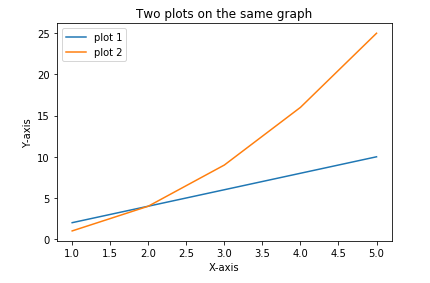
\includegraphics[width=0.75\linewidth]{IMG/mpl.png}
	\label{fig:Mlp}
	\caption{Ảnh minh họa}
\end{figure}
}

\frame{
	\frametitle{Referrences}
	\begin{thebibliography}{1}
		\bibitem{Goldbach1742}[Goldbach, 1742]
		Christian Goldbach.
		\newblock A problem we should try to solve before the ISPN ’43 deadline,
		\newblock \emph{Letter to Leonhard Euler}, 1742.
	\end{thebibliography}
	
}

\frame{
	\frametitle{citation}
	\begin{block}{Open Questions}
		Is every even number the sum of two primes?
		\cite{Goldbach1742}
	\end{block}
	
}



\frame{
    \begin{center}
        \huge \color{blue} \textbf{Bản chất \& Hiện tượng}
    \end{center}
}
\frame{
		\frametitle{Beamer}
		\begin{block}{Mathematics}
         $J = \frac{{\partial (x,y,z)}}{{\partial (u,v,w)}} = \left| {\begin{array}{*{20}{c}}
            {x{'_u}}&{x{'_v}}&{x{'_w}}\\
            {y{'_u}}&{y{'_v}}&{y{'_w}}\\
            {z{'_u}}&{z{'_v}}&{z{'_w}}
        \end{array}} \right|$\\
        $\iiint\limits_V {f(x,y,z)dxdydz = \iiint\limits_{Vuvw} {f.\left| J \right|}}dudvdw$\\
        \end{block}
        \begin{block}{Average}
            \[f\left( {{M_0}} \right) = \frac{1}{{V(\Omega )}}\iiint\limits_\Omega  {f(x,y,z)dxdydz}\]
        \end{block}

}

\frame{
    \begin{center}
        \huge \color{blue} \textbf{Nội Dung \& Hình thức}
    \end{center}
}

\frame{
    \begin{center}
        \huge \color{blue} \textbf{Tất yếu \& Ngẫu nhiên}
    \end{center}
}

\frame{
    \begin{center}
        \huge \color{blue} \textbf{Khả năng \& Hiện thực}
    \end{center}
}
%%%%%%%%%%%%%%%%%%%%%%%%%%%%%%%%%%%%%%%%%%%%%%%%%%%%%%%%%%%%%%%%%%%%%
%%%%%%%%%%%%%%%%%%%%%%%%%%%%%%%%%%%%%%%%%%%%%%%%%%%%%%%%%%%%%%%%%%%%%
\end{document}
\frame
{
  \frametitle{Probability}	
\begin{block}{Mathematics}
abc
$ \ [f\left( {{M_0}} \right) = \frac{1}{{V(\Omega )}} \ ]$
\end{block}
}

